

\chapter{Integração}\label{cap_integracao}
\thispagestyle{fancy}

\begin{flushright}
  [Vídeo] | [Áudio] | \href{https://phkonzen.github.io/notas/contato.html}{[Contatar]}
\end{flushright}

Neste capítulo, estudamos métodos numéricos para a integração de funções reais.

\section{Integração Autoadaptativa}\label{cap_integracao_sec_autoadapt}

Vamos considerar o problema de integrar
\begin{equation}
  I(a,b) = \int_a^b f(x)\,dx
\end{equation}
pela \emph{Regra de Simpson}\footnote{Consulte mais sobre a Regra de Simpson em \href{https://phkonzen.github.io/notas/MatematicaNumerica/cap_integr_sec_NC.html}{Seção 10.1 Regras de Newton-Cotes}.}. Em um dado subintervalo $[\alpha, \beta]\subset [a, b]$, temos
\begin{equation}
  I(\alpha, \beta) = \underbrace{\frac{h_0}{3}\left[f(\alpha) + 4f(\alpha+h_0) + f(\beta)\right]}_{S(\alpha,\beta)}-\frac{h_0^5}{90}f^{(4)}(\xi),
\end{equation}
onde $h_0=(\beta-\alpha)/2$ e $\xi\in (\alpha, \beta)$. Ou seja, temos que
\begin{equation}\label{eq:estS1}
  I(\alpha,\beta) - S(\alpha,\beta) = -\frac{h_0^5}{90}f^{(4)}(\xi).
\end{equation}
A ideia é explorarmos esta informação de forma a obtermos uma estimativa para o erro de integração no intervalo $[\alpha,\beta]$ sem necessitar computar $f^{(4)}$.

Aplicando a Regra de Simpson na partição $[\alpha,(\alpha+\beta)/2]\cup [(\alpha+\beta)/2, \beta]$, obtemos
\begin{equation}
  I(\alpha,\beta) - S_2(\alpha,\beta) = -\frac{(h_0/2)^5}{90}\left(f^{(4)}(\xi) + f^{(4)}(\eta)\right),
\end{equation}
onde $\xi\in (\alpha,(\alpha+\beta)/2)$, $\eta\in (\alpha+\beta)/2, \beta)$ e
\begin{equation}
  S_2(\alpha,\beta) = S(\alpha,(\alpha+\beta)/2) + S((\alpha+\beta)/2,\beta).
\end{equation}
Agora, \emph{vamos assumir que} $f^{(4)}(\xi)\approx f^{(4)}(\eta)$ de forma que temos
\begin{equation}\label{eq:estS2}
  I(\alpha,\beta) - S_2(\alpha,\beta) \approx -\frac{1}{16}\frac{h_0^5}{90}f^{(4)}(\xi).
\end{equation}
De \eqref{eq:estS1} e \eqref{eq:estS2}, obtemos
\begin{equation}
  \frac{h_0^5}{90}f^{(4)}(\xi) \approx \frac{16}{15}\underbrace{\left[S(\alpha,\beta)-S_2(\alpha,\beta)\right]}_{\mathcal{E}(\alpha,\beta)}.
\end{equation}
Isto nos fornece a seguinte estimativa {\it a posteriori} do erro
\begin{equation}
  |I(\alpha,\beta)-S_2(\alpha,\beta)| \approx \frac{|\mathcal{E}(\alpha,\beta)|}{15}.
\end{equation}
Na prática, costuma-se utilizar a seguinte estimativa mais restrita
\begin{equation}
  |I(\alpha,\beta)-S_2(\alpha,\beta)| \approx \frac{|\mathcal{E}(\alpha,\beta)|}{10}.
\end{equation}
Para garantir uma precisão global em $[a,b]$ igual a uma dada tolerância, é suficiente impor que
\begin{equation}
  \frac{|\mathcal{E}(\alpha,\beta)|}{10} \leq \epsilon\frac{\beta-\alpha}{b-a}.
\end{equation}

\lstinputlisting[caption=Algoritmo Simpson Autoadaptativo, label={lst:algSimAd}]{./cap_integracao/dados/pySimAd/main.py}

\begin{ex}
  \begin{align}
    \int_{-3}^4\arctg(10x)\,dx &= -3\arctg(30) - \frac{\ln(1601)}{20} + \frac{\ln(901)}{20} + 4\arctg(40)\\
                               &\approx 1.54203622
  \end{align}
\end{ex}

\begin{exer}
  Implemente uma abordagem autoadaptativa usando a Regra do Trapézio. Valide-a e compare com o exemplo anterior.
\end{exer}

\section{Integrais múltiplas}\label{cap_integracao_sec_intmul}

Vamos trabalhar com métodos para a computação de integrais múltiplas
\begin{equation}
  \int\int_R f(x,y)\,dA.
\end{equation}
Em uma região retangular $A=[a,b]\times [c,d]$, podemos reescrevê-la como uma \emph{integral iterada}
\begin{equation}
  \int\int_R f(x,y)\,dA = \int_a^b\int_c^d f(x,y)\,dy\,dx.
\end{equation}

\subsection{Regras de Newton-Cotes}

\subsubsection{Regra do Trapézio}

A Regra do Trapézio\footnote{\href{https://phkonzen.github.io/notas/MatematicaNumerica/cap_integr_sec_NC.html}{Notas de Aula - Matemática Numérica}.} nos fornece
\begin{equation}
  \int_c^d f(x,y)\,dy = \frac{h_y}{2}\left[f(x,c) + f(x,d)\right] - \frac{h_y^3}{12}f''(x,\eta)
\end{equation}
com $h_y = (d-c)$ e $\eta\in (c,d)$. De forma iterada, temos
\begin{align}
  \int_a^b\int_c^d f(x,y)\,dy\,dx &= \frac{h_y}{2}\int_a^b f(x,c)\,dx + \frac{h_y}{2}\int_a^bf(x,d)\,dx\\
                                  &- \frac{h_y^3}{12}\int_a^b f''(x,\eta)\,dx.
\end{align}
Então, à exceção do termo do erro, aplicamos a Regra do Trapézio para as integrais em $x$. Obtemos
\begin{align}
  \int_a^b\int_c^d f(x,y)\,dy\,dx &= \frac{h_y}{2}\frac{h_x}{2}\left[f(a,c) + f(b,c)\right]\\
                                  &+ \frac{h_y}{2}\frac{h_x}{2}\left[f(a,d) + f(b,d)\right]\\
                                  &-\frac{h_y}{2}\frac{h_x^3}{12}f''(\mu',c)\\
                                  &-\frac{h_y}{2}\frac{h_x^3}{12}f''(\mu'',d)\\
                                  &-\frac{h_y^3}{12}\int_a^b f''(x,\eta)\,dx,
\end{align}
com $h_x = (b-a)$, $\mu',\mu''\in (a,b)$. Pelos Teorema do Valor Intermediário e pelo Teorema do Valor Médio, podemos ver que o erro é $O(h_xh_y^3 + h_x^3h_y)$. Por fim, obtemos a Regra do Trapézio para Integrais Iteradas
\begin{align}
  \int_a^b\int_c^d f(x,y)\,dy\,dx &= \frac{h_y}{2}\frac{h_x}{2}\left[f(a,c)+f(b,c)+f(b,d)+f(a,d)\right]\\
                                  &+ O(h_xh_y^3 + h_x^3h_y).
\end{align}

\begin{ex}
  A Regra do Trapézio fornece
  \begin{equation}
    \int_{1.5}^{2}\int_{1}^{1.5}\ln(x + 2y)\,dy\,dx \approx 0.36.
  \end{equation}
  Verifique!
\end{ex}

\subsubsection{Regra de Simpson}

A Regra do Simpson\footnote{\href{https://phkonzen.github.io/notas/MatematicaNumerica/cap_integr_sec_NC.html}{Notas de Aula - Matemática Numérica}.} nos fornece
\begin{align}
  \int_c^d f(x,y)\,dy &= \frac{h_y}{3}\left[f(x,y_1) + 4f(x,y_2) + f(x,y_3)\right] \\
                      &- \frac{h_y^5}{90}f^{(4)}(x,\eta)
\end{align}
com $h_y = (d-c)/2$, $y_j=(j-1)h_y$, $j=1,2,3$, e $\eta\in (c,d)$. De forma iterada, temos
\begin{align}
  \int_a^b\int_c^d f(x,y)\,dy\,dx &= \frac{h_y}{3}\left[\int_a^bf(x,y_1)\,dx + 4\int_a^bf(x,y_2)\,dx + \int_a^bf(x,y_3)\,dx\right] \\
                                  &- \frac{h_y^5}{90}\int_a^bf^{(4)}(x,\eta)\,dx
\end{align}
Então, à exceção do termo do erro, aplicamos a Regra de Simpson para as integrais em $x$. Obtemos
\begin{align}
  \int_a^b\int_c^d f(x,y)\,dy\,dx &= \frac{h_xh_y}{9}\left[f(x_1,y_1) + 4f(x_2,y_1) + f(x_3,y_1)\right] \\
                                  &+ \frac{4h_xh_y}{9}\left[f(x_1,y_2) + 4f(x_2,y_2) + f(x_3,y_2)\right] \\
                                  &+ \frac{h_xh_y}{9}\left[f(x_1,y_3) + 4f(x_2,y_3) + f(x_3,y_3)\right] \\
                                  &- \frac{h_x^5h_y}{270}f^{(4)}(\mu_1,y_1)\\
                                  &- \frac{4h_x^5h_y}{270}f^{(4)}(\mu_2,y_2)\\
                                  &- \frac{h_x^5h_y}{270}f^{(4)}(\mu_3,y_3) \\
                                  &- \frac{h_y^5}{90}\int_a^bf^{(4)}(x,\eta)\,dx
\end{align}
com $h_x = (b-a)/2$, $\mu_1,\mu_2,\mu_3\in (a,b)$. Pelos Teorema do Valor Intermediário e Teorema do Valor Médio, podemos ver que o erro é $O(h_xh_y^5 + h_x^5h_y)$. Por fim, obtemos a \emph{Regra de Simpson para Integrais Iteradas}
\begin{align}
  \int_a^b\int_c^d f(x,y)\,dy\,dx &= \frac{h_xh_y}{9}\left[f(x_1,y_1) + 4f(x_2,y_1) + f(x_3,y_1)\right] \\
                                  &+ \frac{4h_xh_y}{9}\left[f(x_1,y_2) + 4f(x_2,y_2) + f(x_3,y_2)\right] \\
                                  &+ \frac{h_xh_y}{9}\left[f(x_1,y_3) + 4f(x_2,y_3) + f(x_3,y_3)\right] \\
                                  &+ O(h_xh_y^5 + h_x^5h_y).
\end{align}

\begin{ex}
  A Regra de Simpson fornece
  \begin{equation}
    \int_{1.5}^{2}\int_{1}^{1.5}\ln(x + 2y)\,dy\,dx \approx 0.361003.
  \end{equation}
  Verifique!
\end{ex}

\subsection{Regras Compostas de Newton-Cotes}

A ideia é particionar a região de integração em células e o resultado da integração é a soma da aplicação da regra de quadratura em cada uma das células.

\subsubsection{Regra Composta do Trapézio}

Para uma região retangular $R = [a,b]\times [c,d]$, vamos construir a malha
\begin{equation}
  M = \{c_k=[x_i,x_{i+1}]\times [y_j,y_{j+1}]:~k=i + (j-1)n_x\},
\end{equation}
onde $x_i=(i-1)h_x$, $h_x = (b-a)/n_x$, $i=1,2,\dotsc,n_x+1$ e $y_j=(j-1)h_y$, $h_y=(d-c)/n_y$, $j=1,2,\dotsc,n_y+1$. Consulte a Figura \ref{fig:malhaTrap}.

\begin{figure}[H]
  \centering
  \includegraphics{./cap_integracao/dados/figMalhaTrap/fig}
  \caption{Representação da malha para a Regra Composta do Trapézio.}
  \label{fig:malhaTrap}
\end{figure}

Aplicando a ideia, temos
\begin{align}
  \int_a^b\int_c^d f(x,y)\,dy\,dx &= \sum_{k=1}^{n_xn_y}\int\int_{C_k} f(x,y)\,dy\,dx\\
                                  &= \sum_{i=1}^{n_x}\sum_{j=1}^{n_y}\int_{x_i}^{x_{i+1}}\int_{y_j}^{y_{j+1}} f(x,y)\,dy\,dx
\end{align}
Em cada integral em $C_k$, aplicamos a Regra do Trapézio, segue
\begin{align}
  \int_{x_i}^{x_{i+1}}\int_{y_j}^{y_{j+1}} f(x,y)\,dy\,dx &\approx \frac{h_y}{2}\frac{h_x}{2}\left[f(x_i,y_j) + f(x_{i+1},y_j)\right.\\
                                                          &+ \left.f(x_{i+1},y_{j+1}) + f(x_{i+1},y_{j})\right]
\end{align}
Observamos que nos conjuntos de nodos (marcados em azul na Figura \ref{fig:malhaTrap})
\begin{gather}
  \{(i,j):~i=2,\dotsc,n_x,j=1\text{ ou }j=n_y+1\},\\
  \{(i,j):~i=1\text{ ou }i=n_x+1,j=2,\dotsc,n_y\}
\end{gather}
a função integranda será avaliada $2$ vezes. Já, em todos os nodos internos, $i=2,\dotsc,n_x$, $j=2,\dotsc,n_y$, a função será avaliada $4$ vezes. Com isso, chegamos à Regra Composta do Trapézio
\begin{align}
  \int_a^b\int_c^d f(x,y)\,dy\,dx &= \frac{h_xh_y}{4}\left[f(x_1,y_1)+f(x_{n_x+1},y_1)\right.\nonumber\\
                                  &\left. + f(x_{n_x+1},y_{n_y+1})+f(x_{1},y_{n_y+1})\right]\nonumber\\
                                  &+ \frac{h_xh_y}{2}\sum_{i=2}^{n_x}\left[f(x_i,y_1) + f(x_i,y_{n_y+1})\right]\nonumber\\
                                  &+ \frac{h_xh_y}{2}\sum_{j=2}^{n_y}\left[f(x_1,y_j) + f(x_{n_x+1},y_j)\right]\nonumber\\
                                  &+ h_xh_y\sum_{i=2}^{n_x}\sum_{j=2}^{n_y}f(x_i,y_j)\nonumber\\
                                  &+ O(h_x^2 + h_y^2)
\end{align}
Observamos que esta é uma quadratura de $(n_x+1)(n_y+1)$ nodos.

\begin{exer}
  Verifique a aplicação da Regra Composta do Trapézio para computar
  \begin{equation}
    \int_{1.5}^{2}\int_{1}^{1.5}\ln(x + 2y)\,dy\,dx.
  \end{equation}
\end{exer}

\subsubsection{Regra Composta de Simpson}

Aqui, vamos construir uma malha
\begin{equation}
  M = \left\{C_k = [x_i,x_{i+2}]\times[y_j,y_{j+2}]:~i=1,3,\dotsc,n_x-1, j=1,3,\dotsc,n_y-1,~\right\},
\end{equation}
onde $x_i=(i-1)h_x$, $h_x=(b-a)/n_x$, $i=1,2,\dotsc,n_x+1$ e $y_j=(j-1)h_y$, $h_y=(d-c)/n_y$, $j=1,2,\dotsc,n_y+1$. Com $n_x,n_y\leq 2$ números pares. Consulte a Figura \ref{fig:malhaSim}.

\begin{figure}[H]
  \centering
  \includegraphics{./cap_integracao/dados/figMalhaSim/fig}
  \caption{Representação da malha para a Regra Composta de Simpson.}
  \label{fig:malhaSim}
\end{figure}

A Regra Composta de Simpson para Integrais Iteradas fica
\begin{align}
  \int_a^b\int_c^d f(x,y)\,dx\,dy &= \frac{h_xh_y}{9}\left\{f(x_1,y_1) + f(x_{n_x+1},y_1)\right.\nonumber\\
                                  &+ f(x_1,y_{n_y+1}) + f(x_{n_x+1},y_{n_y+1})\nonumber\\
                                  &+ 2\sum_{i=1}^{n_x/2-1} \left[f(x_{2i+1},y_{1}) + f(x_{2i+1},y_{n_y+1})\right]\nonumber\\
                                  &+ 2\sum_{j=1}^{n_y/2-1} \left[f(x_{1},y_{2j+1}) + f(x_{n_x+1},y_{2j+1})\right]\nonumber\\
                                  &+ 4\sum_{i=1}^{n_x/2} \left[f(x_{2i},y_{1}) + f(x_{2i},y_{n_y+1})\right]\nonumber\\
                                  &+ 4\sum_{j=1}^{n_y/2} \left[f(x_{1},y_{2j}) + f(x_{n_x+1},y_{2j})\right]\nonumber\\
                                  &+ 4\sum_{i=1}^{n_x/2-1}\sum_{j=1}^{n_y/2-1}f(x_{2j+1},y_{2j+1})\nonumber\\
                                  &+ 8\sum_{i=1}^{n_x/2-1}\sum_{j=1}^{n_y/2}f(x_{2i+1},y_{2j})\nonumber\\
                                  &+ 8\sum_{i=1}^{n_x/2}\sum_{j=1}^{n_y/2-1}f(x_{2i},y_{2j+1})\nonumber\\
                                  &\left.+ 16\sum_{i=1}^{n_x/2}\sum_{j=1}^{n_y/2}f(x_{2i},y_{2j})\right\}\nonumber\\
                                  &+ O(h_x^4 + h_y^4).
\end{align}


\begin{exer}
  Verifique a aplicação da Regra Composta de Simpson para computar
  \begin{equation}
    \int_{1.5}^{2}\int_{1}^{1.5}\ln(x + 2y)\,dy\,dx.
  \end{equation}
\end{exer}
